\documentclass[a4paper, 12pt]{article}

%preambles
\usepackage[]{color}

% Include images
\usepackage{graphicx}

% HTTP links in the doc
\usepackage{hyperref}

% For drawing flow graph, arrows
\usepackage{tikz}
\usetikzlibrary{shapes.geometric, arrows}
\usepackage{array,booktabs}
\usepackage{varwidth}
\usepackage{mathtools}


% Inits
\newcommand{\HRule}{\rule{\linewidth}{0.5mm}}
\tikzstyle{startstop} = [rectangle, rounded corners, minimum width=3cm, minimum height=0.9cm,text centered, draw=black]
\tikzstyle{io} = [trapezium, trapezium left angle=70, trapezium right angle=110, minimum width=3cm, minimum height=0.9cm, text centered, draw=black]
\tikzstyle{process} = [rectangle, minimum width=3cm, minimum height=0.9cm, text centered, draw=black]
\tikzstyle{decision} = [diamond, minimum width=3cm, minimum height=0.9cm, text centered, draw=black]
\tikzstyle{arrow} = [thick,->,>=stealth]
\newcolumntype{M}{>{\begin{varwidth}{4cm}}l<{\end{varwidth}}} %M is for Maximal column
\newcommand{\tab}{\-\ \hspace{.5cm}}

\begin{document}
\pagenumbering{roman}
\begin{titlepage}
\begin{center}

~\\[3cm]
\textsc{\Large Analysis and Optimisation of Embedded Systems,
SoSe 2015}\\[1.5cm]

% Title
\HRule \\[0.5cm]
{ \huge \bfseries Exercise 2 \\[0.4cm] }
\HRule \\[0.5cm]
\textbf{Due date: July 02, 2015}

\vfill
\begin{flushleft}
\textbf{Submitted by} \\[0.3cm]
Rajibul Alam, 
\href{mailto:r.alam@campus.tu-berlin.de}{r.alam@campus.tu-berlin.de} \\
Tamilselvan Shanmugam, 
\href{mailto:tamilselvan@mailbox.tu-berlin.de}{tamilselvan@mailbox.tu-berlin.de} \\
Xu CAO,
\href{mailto:xu.cao@campus.tu-berlin.de}{xu.cao@campus.tu-berlin.de} \\
\end{flushleft}

\vspace{1cm}
% Bottom of the page
\begin{flushright}
{\large Last Modified: \today}
\end{flushright}
\end{center}

\end{titlepage}

\pagenumbering{arabic}

\section{Available Expressions Analysis}
\subsection{Control flow graph}
~\\
\begin{center}
	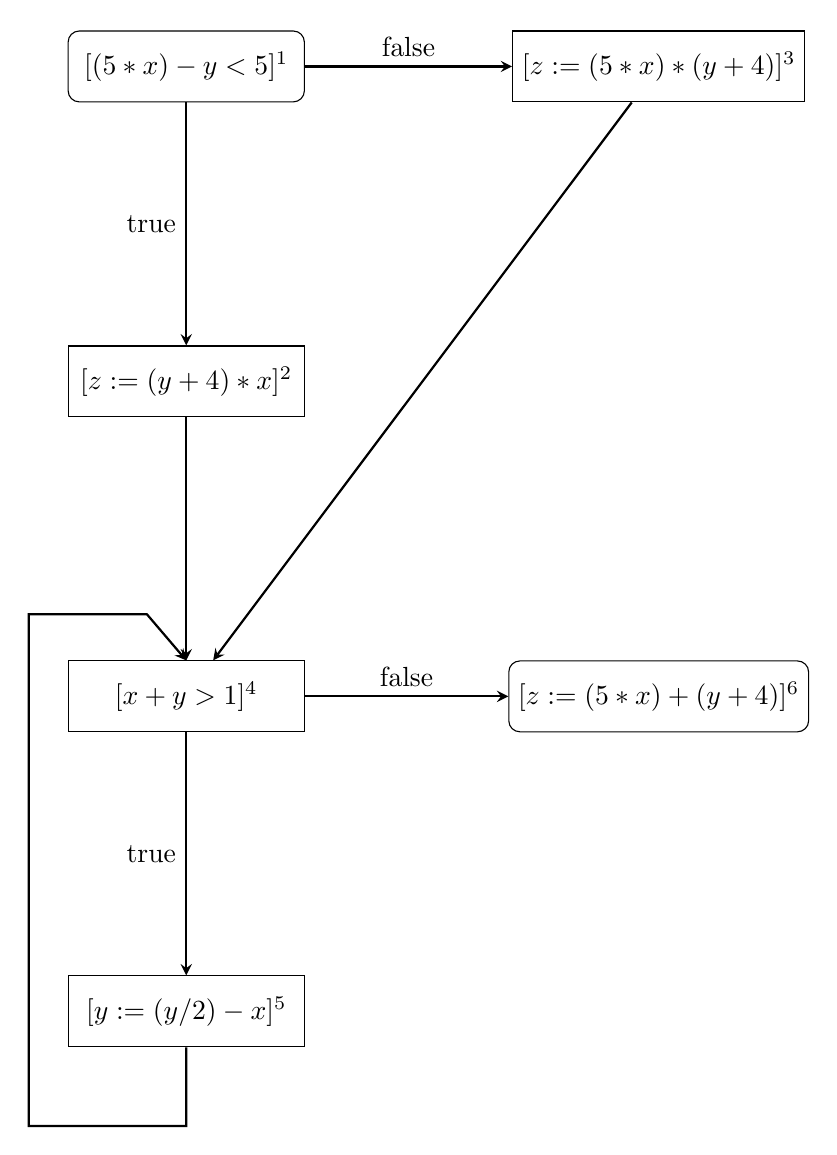
\begin{tikzpicture}[node distance=2cm]
	\node (dec1) [startstop] { $[(5*x)-y < 5]^1$ };
	\node (pro3) [process, right of=dec1, xshift=4cm] { $[z:=(5*x)*(y+4)]^3$ };
	\node (pro2) [process, below of=dec1, yshift=-2cm] { $[z:=(y+4)*x]^2$ };
	\node (pro4) [process, below of=pro2, yshift=-2cm] { $[x+y > 1]^4$ };
	\node (pro5) [process, below of=pro4, yshift=-2cm] { $[y:=(y/2)-x]^5$ };
	\node (stop) [startstop, right of=pro4, xshift=4cm] { $[z:=(5*x)+(y+4)]^6$ };
	\draw [arrow] (dec1) -- node[anchor=east] {true} (pro2);
	\draw [arrow] (dec1) -- node[anchor=south] {false} (pro3);
	\draw [arrow] (pro3) -- (pro4);
	\draw [arrow] (pro2) -- (pro4);
	\draw [arrow] (pro4) -- node[anchor=east] {true} (pro5);
	\draw [arrow] (pro4) -- node[anchor=south] {false} (stop);
	\draw [arrow] (pro5.south) -- ++(0,-1) -- ++(-2,0) -- ++(0,6.5) -- ++(1.5,0) -- (pro4.north);
	\end{tikzpicture}
\end{center}

\subsection{AExp$_*$}
Available expression for the given program is : \textbf{(5*x)} which is computed and not modified throught the program.

\subsection{\textit{kill} and \textit{gen} table}
\begin{center}
	\begin{tabular}{| >{\centering\arraybackslash} m{2cm} | >{\centering\arraybackslash} m{6cm} | >{\centering\arraybackslash} m{4cm} |} 
		\hline
		\textit{l} & kill$_A$$_E$(\textit{l}) & gen$_A$$_E$(\textit{l}) \\
		\hline
		1 & $\emptyset$ & $\lbrace$ (5*x), ((5*x)-y) $\rbrace$ \\
		\hline
		2 & $\emptyset$ & $\lbrace$ (y+4), ((y+4)*x) $\rbrace$ \\
		\hline
		3 & $\emptyset$ & $\lbrace$ (5*x), (y+4), ((5*x)*(y+4)) $\rbrace$ \\
		\hline
		4 & $\emptyset$ & $\lbrace$ (x+y) $\rbrace$ \\[0.25cm]
		\hline
		5 & $\lbrace$ (x+y), (y+4), ((5 * x)*(y+4)), ((y+4)*x), ((5*x)-y), (y/2), ((y/2)-x) $\rbrace$ & $\emptyset$ \\
		\hline
		6 & $\emptyset$ & $\lbrace$ (5*x), (y+4), ((5*x)+(y+4)) $\rbrace$ \\
		\hline
	\end{tabular}
\end{center} ~\\

\subsection{Equation system}
AE$_\circ$(1) = $\emptyset$ \\
AE$_\circ$(2) = AE$_\bullet$(1) \\
AE$_\circ$(3) = AE$_\bullet$(1) \\
AE$_\circ$(4) = AE$_\bullet$(2) $\cap$ AE$_\bullet$(3) $\cap$ AE$_\bullet$(5) \\
AE$_\circ$(5) = AE$_\bullet$(4) \\
AE$_\circ$(6) = AE$_\bullet$(4) \\ \\
AE$_\bullet$(1) = AE$_\circ$(1) $\cup$ $\lbrace$ (5*x), ((5*x)-y) $\rbrace$ \\
AE$_\bullet$(2) = AE$_\circ$(2) $\cup$ $\lbrace$ (y+4), ((y+4)*x) $\rbrace$ \\
AE$_\bullet$(3) = AE$_\circ$(3) $\cup$ $\lbrace$ (5*x), (y+4), ((5*x)*(y+4)) $\rbrace$ \\
AE$_\bullet$(4) = AE$_\circ$(4) $\cup$ $\lbrace$ (x+y) $\rbrace$ \\
AE$_\bullet$(5) = AE$_\circ$(5) \textbackslash(x+y), (y+4), ((5 * x)*(y+4)), ((y+4)*x), \\ 
\tab \tab \tab ((5*x)-y), (y/2), ((y/2)-x) $\cup$ $\emptyset$ \\
AE$_\bullet$(6) = AE$_\circ$(6) $\cup$ $\lbrace$ (5*x), (y+4), ((5*x)+(y+4)) $\rbrace$ \\

\subsection{Simplifying Equation}
\textbf{Let us consider}
\begin{flalign*}% left aligned
	a &= 5*x &\\
	b &= (5*x)-y &\\
	c &= y+4 &\\
	d &= (y+4)*x &\\
	e &= (5*x)*(y+4) &\\
	f &= x+y &\\
\end{flalign*}
\textbf{Solution}
\begin{flalign*}% left aligned
	AE_\circ(1) &= \emptyset &\\
	AE_\bullet(1) &= \lbrace a,b \rbrace &\\ \\
	AE_\circ(2) &= \lbrace a,b \rbrace &\\
	AE_\bullet(2) &= \lbrace a,b,c,d \rbrace &\\ \\
	AE_\circ(3) &= \lbrace a,b \rbrace &\\
	AE_\bullet(3) &= \lbrace a,b,c,e \rbrace &\\ \\
	AE_\circ(4) &= \lbrace a,b,c,d \rbrace \cap \lbrace a,b,c,e \rbrace \cap AE_\bullet(5) &\\
	&= \lbrace a,b,c \rbrace \cap AE_\bullet(5) &\\
	AE_\bullet(4) &= \lbrace a,b,c \rbrace \cap AE_\bullet(5) \cup \lbrace f \rbrace &\\ \\
	AE_\circ(5) &= \lbrace a,b,c \rbrace \cap AE_\bullet(5) \cup \lbrace f \rbrace &\\
	AE_\bullet(5) &= (\lbrace a,b,c \rbrace \cap AE_\bullet(5) \cup \lbrace f \rbrace) \backslash \lbrace b,c,d,e,f \rbrace &\\
	&= \lbrace a \rbrace \cap AE_\bullet(5) &\\
\end{flalign*}
Solutions for AE$_\bullet$(5) are \textbf{(5*x)} and \textbf{$\mathbf{\emptyset}$} \\

\subsection{Largest solution}
\begin{center}
	\begin{tabular}{| >{\centering\arraybackslash} m{2cm} | >{\centering\arraybackslash} m{5cm} | >{\centering\arraybackslash} m{5cm} |} 
		\hline
		\textit{l} & AE$_\circ$(\textit{l}) & AE$_\bullet$(\textit{l}) \\
		\hline
		1 & $\emptyset$ & $\lbrace$ (5*x), ((5*x)-y) $\rbrace$ \\
		\hline
		2 & $\lbrace$ (5*x), ((5*x)-y) $\rbrace$ & $\lbrace$ (5*x), ((5*x)-y), (y+4), ((y+4)*x) $\rbrace$ \\
		\hline
		3 & $\lbrace$ (5*x), ((5*x)-y) $\rbrace$ & $\lbrace$ (5*x), ((5*x)-y), (y+4), ((5*x)*(y+4)) $\rbrace$ \\
		\hline
		4 & $\lbrace$ (5*x) $\rbrace$ & $\lbrace$ (5*x), (x+y) $\rbrace$ \\
		\hline
		5 & $\lbrace$ (5*x), (x+y) $\rbrace$ & $\lbrace$ (5*x) $\rbrace$ \\
		\hline
		6 & $\lbrace$ (5*x), (x+y) $\rbrace$ & $\lbrace$ (5*x), (x+y), (y+4), ((5*x)+(y+4)) $\rbrace$ \\
		\hline
	\end{tabular}
\end{center}

\section{Live Variables Analysis}
\subsection{pseudo code of the worklist algorithm $\cite{pseudocode}$}
\textbf{for} all (\textit{v}) \\
\tab OUT(\textit{v}) = $\emptyset$ \\
\tab IN(\textit{v}) = USE(\textit{v}) \\
\textbf{end for} \\
worklist $\longleftarrow$ set of all nodes \\
\textbf{while} (worklist $\neq \emptyset$ ) \\
\tab pick and remove a node \textit{v} from worklist \\
\tab OUT(\textit{v}) = $\underset{s\in SUCC(v)}{\cup}$ IN(\textit{s}) \\
\tab oldin = IN(\textit{v}) \\
\tab IN(\textit{v}) = USE(\textit{v}) $\cup$ (OUT(\textit{v}) - DEF(\textit{v})) \\
\tab \textbf{if} oldin $\neq$ IN(\textit{v}) \\
\tab \tab worklist $\longleftarrow$ worklist $\cup$ PRED(\textit{v}) \\
\textbf{end while}\\

\subsection{Live variable analysis}
Initializing the nodes \\
\begin{center}
	\begin{tabular}{| >{\centering\arraybackslash} m{2cm} | >{\centering\arraybackslash} m{4cm} | >{\centering\arraybackslash} m{2cm} |} 
		\hline
		\textit{l} & IN(\textit{l}) & OUT(\textit{l}) \\
		\hline
		 1 & $\lbrace$ x,y $\rbrace$ & $\emptyset$ \\
		 \hline
		 2 & $\lbrace$ x,y $\rbrace$ & $\emptyset$ \\
		 \hline
		 3 & $\lbrace$ x,y $\rbrace$ & $\emptyset$ \\
		 \hline
		 4 & $\lbrace$ x,y $\rbrace$ & $\emptyset$ \\
		 \hline
		 5 & $\lbrace$ x,y $\rbrace$ & $\emptyset$ \\
		 \hline
		 6 & $\lbrace$ x,y $\rbrace$ & $\emptyset$ \\
		 \hline
	\end{tabular}
\end{center} ~\\
\textbf{W = 1,2,3,4,5,6} \tab \textbf{picked node = 1} \\
\textbf{W = 2,3,4,5,6} \\
\begin{align*}
	OUT(1) &= \lbrace x,y \rbrace \cup \lbrace x,y \rbrace \\
	&= \lbrace x,y \rbrace \\
	oldIn &= \lbrace x,y \rbrace \\
	IN(1) &= \lbrace x,y \rbrace \cup (\lbrace x,y \rbrace - \emptyset) \\
	&= \lbrace x,y \rbrace \\
	oldIn &= IN(1) \\
	W &= \lbrace 2,3,4,5,6 \rbrace \\
\end{align*}
\textbf{picked node = 2} \\
\textbf{W = $\lbrace$ 3,4,5,6 $\rbrace$} \\
\begin{align*}
	OUT(2) &= \lbrace x,y \rbrace \\
	oldIn &= \lbrace x,y \rbrace \\
	IN(2) &= \lbrace x,y \rbrace \cup (\lbrace x,y \rbrace - \lbrace z \rbrace) \\
	&= \lbrace x,y \rbrace \\
	oldIn &= IN(2) \\
	W &= \lbrace 3,4,5,6 \rbrace \\
\end{align*}
\textbf{picked node = 3} \\
\textbf{W = $\lbrace$ 4,5,6 $\rbrace$} \\
\begin{align*}
	OUT(3) &= \lbrace x,y \rbrace \\
	oldIn &= \lbrace x,y \rbrace \\
	IN(3) &= \lbrace x,y \rbrace \cup (\lbrace x,y \rbrace - \lbrace z \rbrace) \\
	&= \lbrace x,y \rbrace \\
	oldIn &= IN(3) \\
	W &= \lbrace 4,5,6 \rbrace \\
\end{align*}
\textbf{picked node = 4} \\
\textbf{W = $\lbrace$ 5,6 $\rbrace$} \\
\begin{align*}
	OUT(4) &= IN(5) \cup IN(6) \\
	&= \lbrace x,y \rbrace \\
	oldIn &= \lbrace x,y \rbrace \\
	IN(4) &= \lbrace x,y \rbrace \cup (\lbrace x,y \rbrace - \emptyset) \\
	&= \lbrace x,y \rbrace \\
	oldIn &= IN(4) \\
	W &= \lbrace 5,6 \rbrace \\
\end{align*}
\textbf{picked node = 5} \\
\textbf{W = $\lbrace$ 6 $\rbrace$} \\
\begin{align*}
	OUT(5) &= \lbrace x,y \rbrace \\
	oldIn &= \lbrace x,y \rbrace \\
	IN(5) &= \lbrace x,y \rbrace \cup (\lbrace x,y \rbrace - \lbrace y \rbrace) \\
	&= \lbrace x,y \rbrace \\
	oldIn &= IN(5) \\
	W &= \lbrace 6 \rbrace \\
\end{align*}
\textbf{worklist W = $\emptyset$} \\
\textbf{picked node = 6, W = $\lbrace$ 5,4,3,2,1, $\rbrace$}
\begin{align*}
	OUT(6) &= \emptyset \\
	oldIn &= \lbrace x,y \rbrace \\
	IN(6) &= \lbrace x,y \rbrace \cup (\emptyset - \lbrace z \rbrace) \\
	&= \lbrace x,y \rbrace \\
	oldIn &= IN(6) \\
	W &= \emptyset \\
\end{align*} 
\textbf{Live variables}
\begin{center}
	\begin{tabular}{| >{\centering\arraybackslash} m{2cm} | >{\centering\arraybackslash} m{4cm} | >{\centering\arraybackslash} m{2cm} |} 
		\hline
		\textit{l} & IN(\textit{l}) & OUT(\textit{l}) \\
		\hline
		 1 & $\lbrace$ x,y $\rbrace$ & $\lbrace$ x,y $\rbrace$ \\
		 \hline
		 2 & $\lbrace$ x,y $\rbrace$ & $\lbrace$ x,y $\rbrace$ \\
		 \hline
		 3 & $\lbrace$ x,y $\rbrace$ & $\lbrace$ x,y $\rbrace$ \\
		 \hline
		 4 & $\lbrace$ x,y $\rbrace$ & $\lbrace$ x,y $\rbrace$ \\
		 \hline
		 5 & $\lbrace$ x,y $\rbrace$ & $\lbrace$ x,y $\rbrace$ \\
		 \hline
		 6 & $\lbrace$ x,y $\rbrace$ & $\emptyset$ \\
		 \hline
	\end{tabular}
\end{center} ~\\

\subsection{Perform the program according to the small-step operational semantics}
\textbf{step0:}\\
\\
$\dfrac{(5*x-y<5,[x=4,y=32,z=3])=tt}{\splitfrac{(if[5*x-y<5]then[z:=(y+4)*4]else[z:=(5*x)*(y+4)], [x=4,y=32,z=3])}{\Rightarrow(z:=(y+4)*x,[x=4,y=32,z=144])}}$
\\
\\
\textbf{step1:}\\
\\
$\dfrac{(x+y>1,[x=4,y=32,z=144])=tt}{\splitfrac{(while[x+y>1]do[y:=(y/2)-x],[x=4,y=32,z=144])}{\Rightarrow([y:=(y/2)-x],while[x+y>1]do[y:=(y/2)-x],[x=4,y=12,z=144])}}$
\\
\\
\textbf{step2:}\\
\\
$\dfrac{(x+y>1,[x=4,y=12,z=144])=tt}{\splitfrac{(while[x+y>1]do[y:=(y/2)-x],[x=4,y=12,z=144])}{\Rightarrow([y:=(y/2)-x],while[x+y>1]do[y:=(y/2)-x],[x=4,y=2,z=144])}}$
\\
\\
\textbf{step3:}\\
\\
$\dfrac{(x+y>1,[x=4,y=2,z=144])=tt}{\splitfrac{(while[x+y>1]do[y:=(y/2)-x],[x=4,y=2,z=144])}{\Rightarrow([y:=(y/2)-x],while[x+y>1]do[y:=(y/2)-x],[x=4,y=-3,z=144])}}$
\\
\\
\textbf{step4:}\\
\\
$\dfrac{(x+y>1,[x=4,y=-3,z=144])=ff}{(while[x+y>1]do[y:=(y/2)-x],[x=4,y=-3,z=144])\Rightarrow([x=4,y=-3,z=144])}$
\\
\\
\textbf{step5:}\\
\\
${(z:=(5*x)+(y+4),[x=4,y=-3,z=144])\Rightarrow([x=4,y=-3,z=21])}$
\\
\\

\section{Verification of Live Variables Analysis}
\subsection{Proof of Lemmas}
\subsubsection{if(S,s)$\Rightarrow$(S$^\prime$,s$^\prime$) then flow(S$^\prime$) $\subseteq$ flow(S)}
\textbf{case:i} \\
$\langle S_1;S_2,s \rangle \rightarrow \langle S_1^\prime;S_2,s\prime \rangle$ because $\langle S_1,s \rangle \rightarrow \langle S_1^\prime, s\prime \rangle$ 
\begin{flalign*}
	flow(S_1,S_2) &= flow(S_1) \cup flow(S_2) \cup \lbrace(l,init(S_2)) | l \in final(S_1) \rbrace & \\
	&\supseteq flow(S_1^\prime) \cup flow(S_2) \cup \lbrace (l,init(S_2)) | l \in final(S_1^\prime) \rbrace &\\
	&= flow(S_1^\prime;S_2) & \\
\end{flalign*}
\textbf{case:ii}
$\langle S_1;S_2,s \rangle \rightarrow \langle S_2,s\prime \rangle$ because $\langle S_1,s \rangle \rightarrow \langle S_2, s\prime \rangle$
\begin{flalign*}
	flow(S_1,S_2) &= flow(S_1) \cup flow(S_2) \cup \lbrace(l,init(S_2)) | l \in final(S_1) \rbrace & \\
	&\supseteq flow(S_2) & \\
\end{flalign*}
\textbf{case:iii} \\
$\langle$if [b]$^l$ then S$_1$ else S$_2$, s$ \rangle \rightarrow \langle$ S$_1$, s $\rangle$ because $B[\![b]\!] = true$ \\
\begin{flalign*}
	flow(if\, [b]^l\, then\, S_1\, else\, S_2,\, s)  &= flow(S_1) \cup flow(S_2) \, \cup \lbrace(l,init(S_1)),(l,init(S_2))\rbrace &\\
	&\supseteq flow(S_1) &\\
\end{flalign*}
\textbf{case:iv} \\
$\langle$if [b]$^l$ then S$_1$ else S$_2$, s$ \rangle \rightarrow \langle$ S$_2$, s $\rangle$ because $B[\![b]\!] = false$ \\
\begin{flalign*}
	flow(if\, [b]^l\, then\, S_1\, else\, S_2,\, s)  &= flow(S_1) \cup flow(S_2) \, \cup \lbrace(l,init(S_1)),(l,init(S_2))\rbrace &\\
	&\supseteq flow(S_2) &\\
\end{flalign*}
\textbf{case:v} \\
$\langle\, while\, [b]^l\, do\, S,s \rangle \rightarrow \langle S;while\, [b]^l\, do\, S,s \rangle$ because B$[\![b]\!]$ = true \\
\begin{flalign*}
	flow(S;while\, [b]^l\, do\, S,s) &= flow(S) \cup flow(while\, [b]^l\, do\, S,s) \cup \lbrace(l^\prime,l) | l^\prime \in final(S) \rbrace &\\
	&= flow(S) \cup flow(S) \cup \lbrace(l,init(S))\rbrace \cup \lbrace(l^\prime,l) | l^\prime \in final(S)\rbrace \\ 
	&\quad \cup \lbrace(l^\prime,l) | l^\prime \in final(S)\rbrace &\\ 
	&= flow(S) \cup \lbrace(l,init(S))\rbrace \cup \lbrace(l^\prime,l) | l^\prime \in final(S)\rbrace &\\
	&= flow(while\, [b]^l\, do\, S) &\\
\end{flalign*}

\subsubsection{if(S,s)$\Rightarrow$(S$^\prime$,s$^\prime$) then blocks(S$^\prime$) $\subseteq$ blocks(S)}
\textbf{case:1} \\
$\langle S_1;S_2,s \rangle \rightarrow \langle S_1^\prime;S_2,s\prime \rangle$ because $\langle S_1,s \rangle \rightarrow \langle S_1^\prime, s\prime \rangle$ 
\begin{flalign*}
	blocks(S_1,S_2) &= blocks(S_1) \cup blocks(S_2) &\\
	&= blocks(S_1^\prime) \cup blocks(S_2) &\\
	&\supseteq blocks(S_1^\prime) &\\
\end{flalign*}
\textbf{case:ii}
$\langle S_1;S_2,s \rangle \rightarrow \langle S_2,s\prime \rangle$ because $\langle S_1,s \rangle \rightarrow \langle S_2, s\prime \rangle$
\begin{flalign*}
	blocks(S_1,S_2) &= blocks(S_1) \cup blocks(S_2) &\\
	&\supseteq blocks(S_2) &\\
\end{flalign*}
\textbf{case:iii} \\
$\langle$if [b]$^l$ then S$_1$ else S$_2$, s$ \rangle \rightarrow \langle$ S$_1$, s $\rangle$ because $B[\![b]\!] = true$ \\
\begin{flalign*}
	blocks(if\, [b]^l\, then\, S_1\, else\, S_2,\, s)  &= blocks(S_1) \cup blocks(S_2)\, \cup \lbrace[b]^l \rbrace &\\
	&\supseteq blocks(S_1) &\\
\end{flalign*}
\textbf{case:iv} \\
$\langle$if [b]$^l$ then S$_1$ else S$_2$, s$ \rangle \rightarrow \langle$ S$_2$, s $\rangle$ because $B[\![b]\!] = false$ \\
\begin{flalign*}
	blocks(if\, [b]^l\, then\, S_1\, else\, S_2,\, s)  &= blocks(S_1) \cup blocks(S_2)\, \cup \lbrace[b]^l \rbrace &\\
	&\supseteq blocks(S_2) &\\
\end{flalign*}
\textbf{case:v} \\
$\langle\, while\, [b]^l\, do\, S,s \rangle \rightarrow \langle S;while\, [b]^l\, do\, S,s \rangle$ because B$[\![b]\!]$ = true \\
\begin{flalign*}
	blocks(S;while\, [b]^l\, do\, S,s) &= blocks(S) \cup blocks(while\, [b]^l\, do\, S) &\\
	&= blocks(S) \cup blocks(S) \cup \lbrace[b]^l\rbrace &\\ 
	&= blocks(S) \cup \lbrace[b]^l\rbrace &\\ 
	&= blocks(while\, [b]^l\, do\, S) &\\
\end{flalign*}

\subsection{Proof of skip and seq composition}
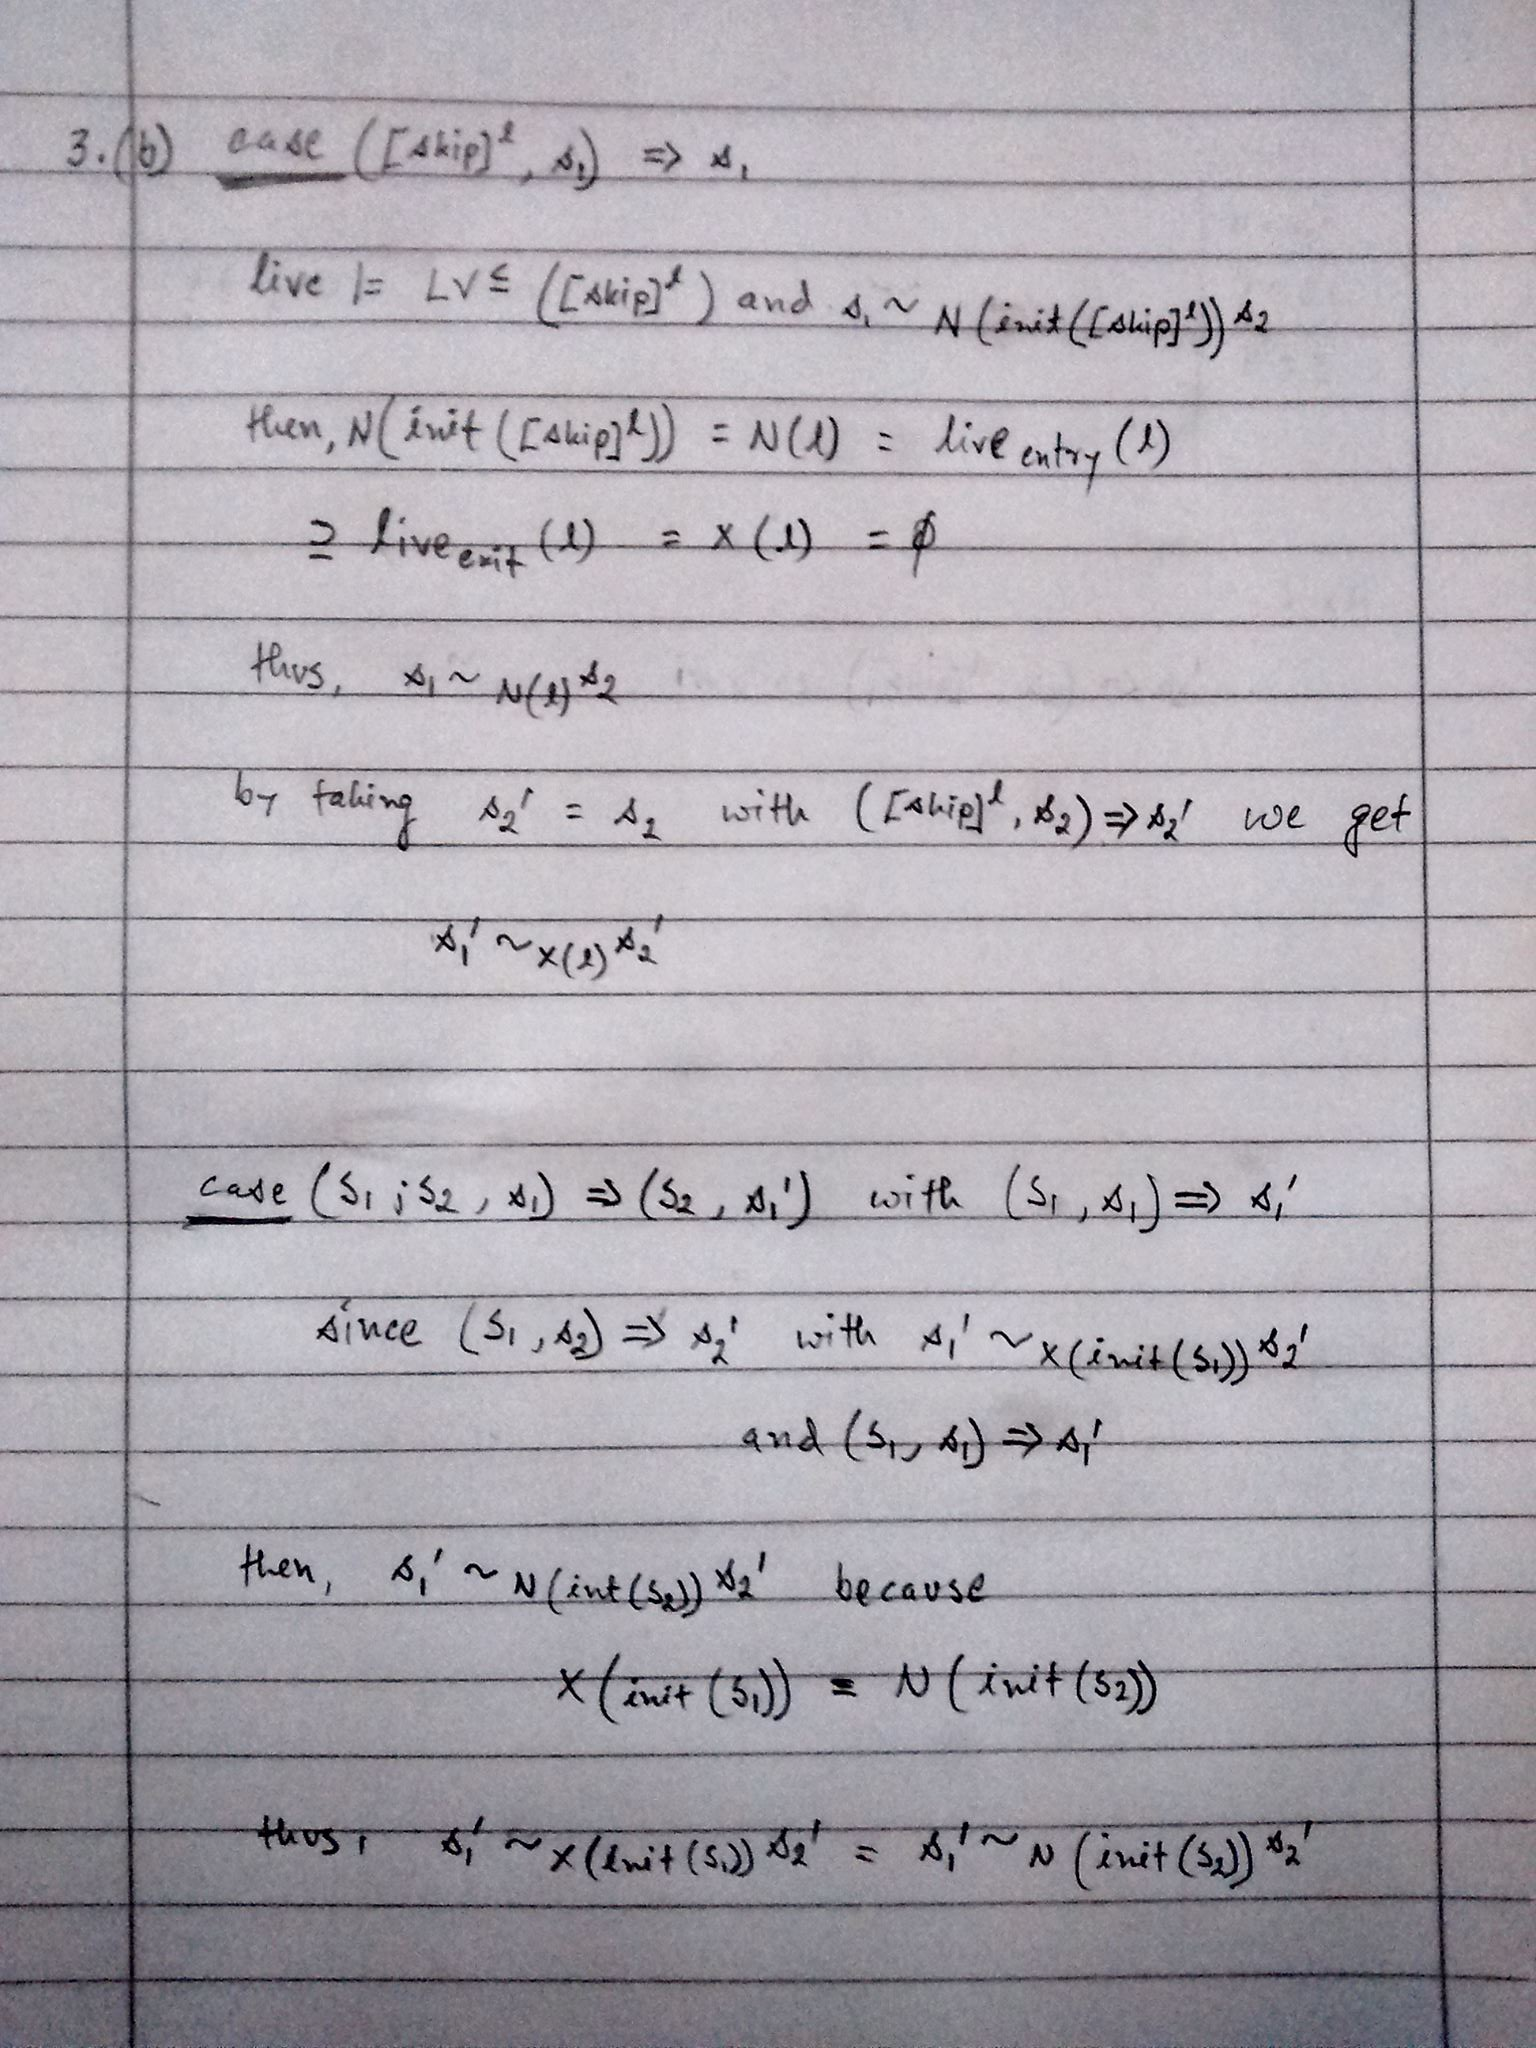
\includegraphics[scale=0.25]{img/3b}

\bibliographystyle{plain}
\bibliography{Solution1}
\end{document}
